% !TEX root = ./main.tex
\section{账本管理的三元悖论}\label{sec:triangle}
根据PFMI的指导原则,金融基础设施应该接受中央银行、市场监管者或者其它管理部门适当、有效的管理、监管和监督。
为了保证金融系统的安全和稳定,各国央行和监管机构对金融机构提出了Know-Your-Customer(KYC)、Anti-Money-Laundering(AML)、Counter-Financing-of-Terrorism (CFT)等合规要求。
但是在实际应用过程中,分布式账本技术在这方面一直比较弱,甚至有些产品的设计目标就是抗审查、抗监管。
从一定程度上助长了洗钱等金融犯罪行为。
根据日本警方报告\cite{jp_report},2018年加密货币洗钱案件增加了十倍。
2017年,日本国家警察局发现了不到700起加密洗钱事件;2018年,他们发现了7,000多起同类案件。

%分布式账本要成为金融基础设施,在保留其技术优势的同时,还要满足金融监管的要求。
分布式账本固有的抗审查性可以用一个三元悖论来解释:

\begin{quotation}
    \textbf{任何独立的账本管理系统只能同时实现以下三个目标中的两个: 去中心化账本管理、账本数据的完整性、账本数据的隐私性。}
\end{quotation}

\begin{figure}[h!]
    \centering
    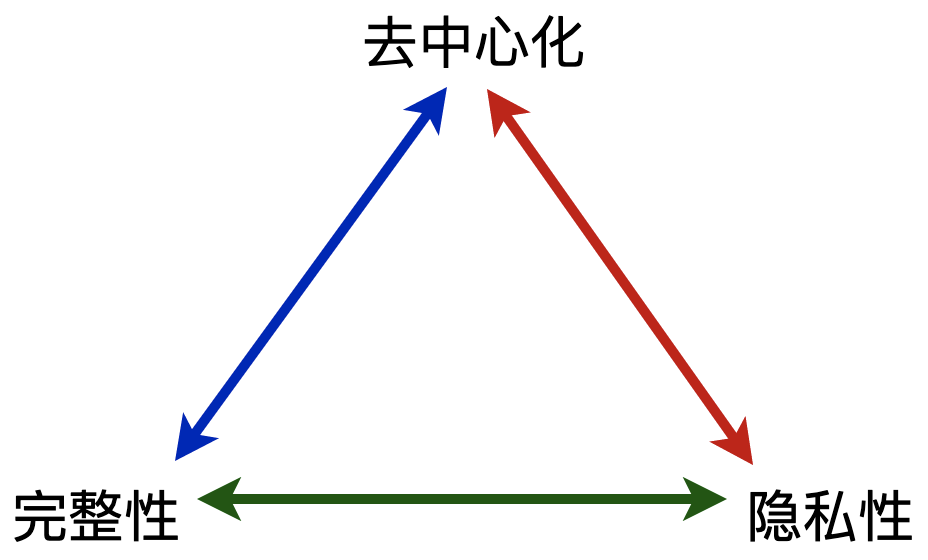
\includegraphics[width=8cm, keepaspectratio]{images/triangle.png}
    \caption{账本数据的三元悖论}
    \label{fig:triangle}
\end{figure}

%这个矛盾的根源在于分布式账本作为共享账本,满足了账本数据的公开性,无法再满足完备性。
%一般来讲,在金融系统中,无论是中心化账本还是去中心化账本,都无法同时满足公开性和完整性。

其中去中心化、完整性、和隐私性的定义如下:
\begin{itemize}
    \item[\dag] \textbf{去中心化}:
    账本数据保存在多个不同的节点中,便于其它节点验证账本数据,同时通过共识机制保证账本数据的一致性。

    \item[\dag] \textbf{完整性}:
    按照PFMI的需求:金融机构或者金融监管方需要完整的身份信息和交易背景信息,以及其它用于验证交易是否合规的真实账户数据。
    
    \item[\dag] \textbf{隐私性}:
    只有交易的参与方与金融监管方才能了解交易的相关隐私数据,其它人员无法根据公开数据推导出交易隐私信息。
\end{itemize}

中心化账本的优势在于可以同时实现完整性和隐私性。与交易相关的隐私数据被集中化管理,不对外公开。在保证隐私性的同时,账本管理者可以利用完整的交易信息做合规审核,监控与防范洗钱等金融犯罪行为。缺点是依赖于账本管理者的信任背书,而且账本之间彼此不透明,提高了金融监管的成本。

去中心化账本的优势在于:账本数据是公开,其它节点可以验证所有交易数据,但是不能同时兼顾完整性和隐私性。
除了一些特殊情况之外\footnote{比如公募慈善基金的资金要接受公众的监督},只能为了保护隐私性而牺牲完整性。
所以分布式账本上的数据都是不完整的,交易记录中只能存储不敏感的数据。导致链上交易数据与真实交易背景信息脱节,无法执行反洗钱等合规审核。

账本数据的不完整性是分布式账本固有的特征,不可能在分布式账本的技术框架内实现。
为了满足各国法律监管合规的要求,必须要创造性的将分布式账本与中心化的账本融合在一起才能找到合适的解决方案。

%目前的主流分布式账本平台普遍无法满足合规、监管需求,具体的来讲,表现在以下几个方面:
%
%\begin{itemize}
%    \item 用户真实身份信息的缺失
%    \item 交易背景数据的缺失
%    \item 交易过程中缺少合规验证环节
%\end{itemize}
